\documentclass[fsharpNotes.tex]{subfiles}
\graphicspath{ {./figures/} }

\begin{document}
\chapter{Common Language Infrastructure}
\label{chap:cli} 
The \idx{Common Language Infrastructure} (\idx{CLI}), not to be confused with \idx{Command Line Interface} with the same acronym, is a technical standard developed by Microsoft \cite{iso23271:2012, ecma335}. The standard specifies a language, its format, and a runtime environment that can execute the code. The main feature is that it provides a common interface between many languages and many platforms, such that programs can collaborate in a language-agnostic manner and can be executed on different platforms without having to be recompiled. Main features of the standard are:
\begin{description}
\item[Common Type System (CTS)]\idxs{Common Type System}\idxs{CTS} which defines a common set of types that can be used across different languages as if it were their own.
\item[Metadata]\idxs{Metadata} which defines a common method for referencing programming structures such as values and functions in a language-independent manner.
\item[Common Intermediate Language (CIL)]\idxs{Common Intermediate Language}\idxs{CIL} which is a platform-independent, stack-based, object-oriented assembly language that can be executed by the Virtual Execution System.
\item[Virtual Execution System (VES)]\idxs{Virtual Execution
    System}\idxs{VES} which is a platform dependent, virtual machine,
  which combines the above into code that can be executed at
  runtime. Microsoft's implementation of VES is called \idx{Common
    Language Runtime} (\idx{CLR}) and uses \idx{just-in-time}
  compilation. In this book, we have been using the
  \lstinline[language=console]{mono} command.
\end{description}
The process of running an F\# program is shown in
\Cref{fig:cliOverview}.
\begin{figure}
  \centering
  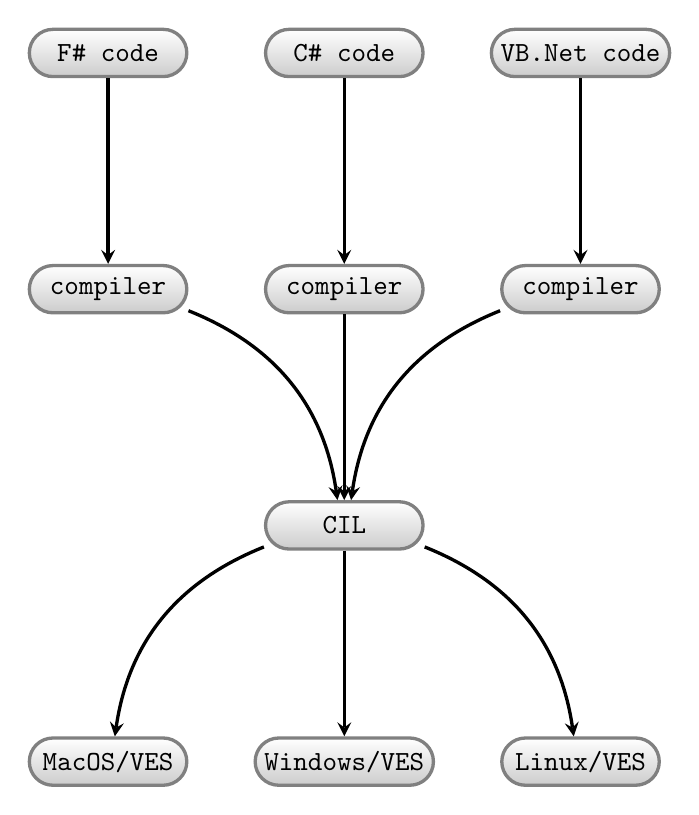
\begin{tikzpicture}[node distance=3cm,
    terminal/.style={
      % The shape:
      rectangle,minimum size=6mm,minimum width=20mm,rounded corners=3mm,
      % The rest
      very thick,draw=black!50,
      top color=white,bottom color=black!20,
      font=\ttfamily}]
    \node (fsharp)  [terminal] {F\# code};
    \node (csharp)  [terminal,right of=fsharp] {C\# code};
    \node (vb)  [terminal,right of=csharp] {VB.Net code};
    \node (fsharpc)  [terminal,below of=fsharp] {compiler}; 
    \node (csharpc)  [terminal,below of=csharp] {compiler}; 
    \node (vbc)  [terminal,below of=vb] {compiler};
    \node (cil)  [terminal,below of=csharpc] {CIL}; 
    \node (win)  [terminal,below of=cil] {Windows/VES}; 
    \node (mac)  [terminal,left of=win] {MacOS/VES}; 
    \node (lin)  [terminal,right of=win] {Linux/VES}; 
    \draw[-stealth,very thick]  (fsharp) edge (fsharpc);
    \draw[-stealth,very thick]  (csharp) edge (csharpc);
    \draw[-stealth,very thick]  (vb) edge (vbc);
    \draw[-stealth,very thick,bend left]  (fsharpc) edge (cil);
    \draw[-stealth,very thick]  (csharpc) edge (cil);
    \draw[-stealth,very thick,bend right]  (vbc) edge (cil);
    \draw[-stealth,very thick,bend right]  (cil) edge (mac);
    \draw[-stealth,very thick]  (cil) edge (win);
    \draw[-stealth,very thick,bend left]  (cil) edge (lin);
  \end{tikzpicture}
  \caption{The relation between some .NET/Mono languages with the
    Common intermediate language (CIL), and the Virtual
    execution systems (VES) on some operating system (\lstinline[language=console]{mono}).}
  \label{fig:cliOverview}
\end{figure}
First the F\# code is compiled or interpreted to CIL. This code possibly combined with other CIL code is then converted to a machine-readable code, and the result is then executed on the platform.


CLI defines a \idx{module} as a single file containing executable code by VES. Hence, CLI's notion of a module is somewhat related to F\#'s notion of module, but the two should not be confused. A collection of modules, a \idx{manifest}, and possibly other resources, which jointly define a complete program is called an \idx{assembly}. The manifest is the description of which files are included in the assembly together with its version, name, security information, and other bookkeeping information.
\end{document}
